\documentclass[10pt,twocolumn,letterpaper]{article}

\usepackage{iccv}
\usepackage{times}
\usepackage{epsfig}
\usepackage{graphicx}
\usepackage{amsmath}
\usepackage{amssymb}
\usepackage{indentfirst}

% Include other packages here, before hyperref.

% If you comment hyperref and then uncomment it, you should delete
% egpaper.aux before re-running latex.  (Or just hit 'q' on the first latex
% run, let it finish, and you should be clear).
\usepackage[breaklinks=true,bookmarks=false]{hyperref}

\iccvfinalcopy % *** Uncomment this line for the final submission

\def\iccvPaperID{****} % *** Enter the ICCV Paper ID here
\def\httilde{\mbox{\tt\raisebox{-.5ex}{\symbol{126}}}}

% Pages are numbered in submission mode, and unnumbered in camera-ready
%\ificcvfinal\pagestyle{empty}\fi
\setcounter{page}{1}
\begin{document}



%%%%%%%%% BODY TEXT
\section{Tracing Neurons}
\subsection{Overview}
To understand the coordinated activity of neurons in brain has become a central goal of neuroscience nowadays. That means we have to know the location of billions of interconnected neurons and understand the connections between them. Obviously, it takes huge amount of time and a lot of effort without a computer-aided system. For most of the 20th century, reconstructing, annotating, and analyzing neurons has been done by creating hand-drawn images of labeled neurons, traced using an instrument known as camera lucida directly from thin brain sections viewed through a microscope[1]. Even some newly developed systems for tracing neurons are reported to have drawbacks like NeuroLucida(the current industry standard for neuron tracing)and TeraFly plugin for Vaa3D. Besides, some automatic techniques for neuron reconstruction will fail on complex and noisy data. The manually process of tracing labeled neuronal connections through the brain should be automated. The difficulties in current systems should be improved with more advanced methods.

\begin{figure}[h]
\begin{center}
%\fbox{\rule{0pt}{2in} \rule{0.9\linewidth}{0pt}}
   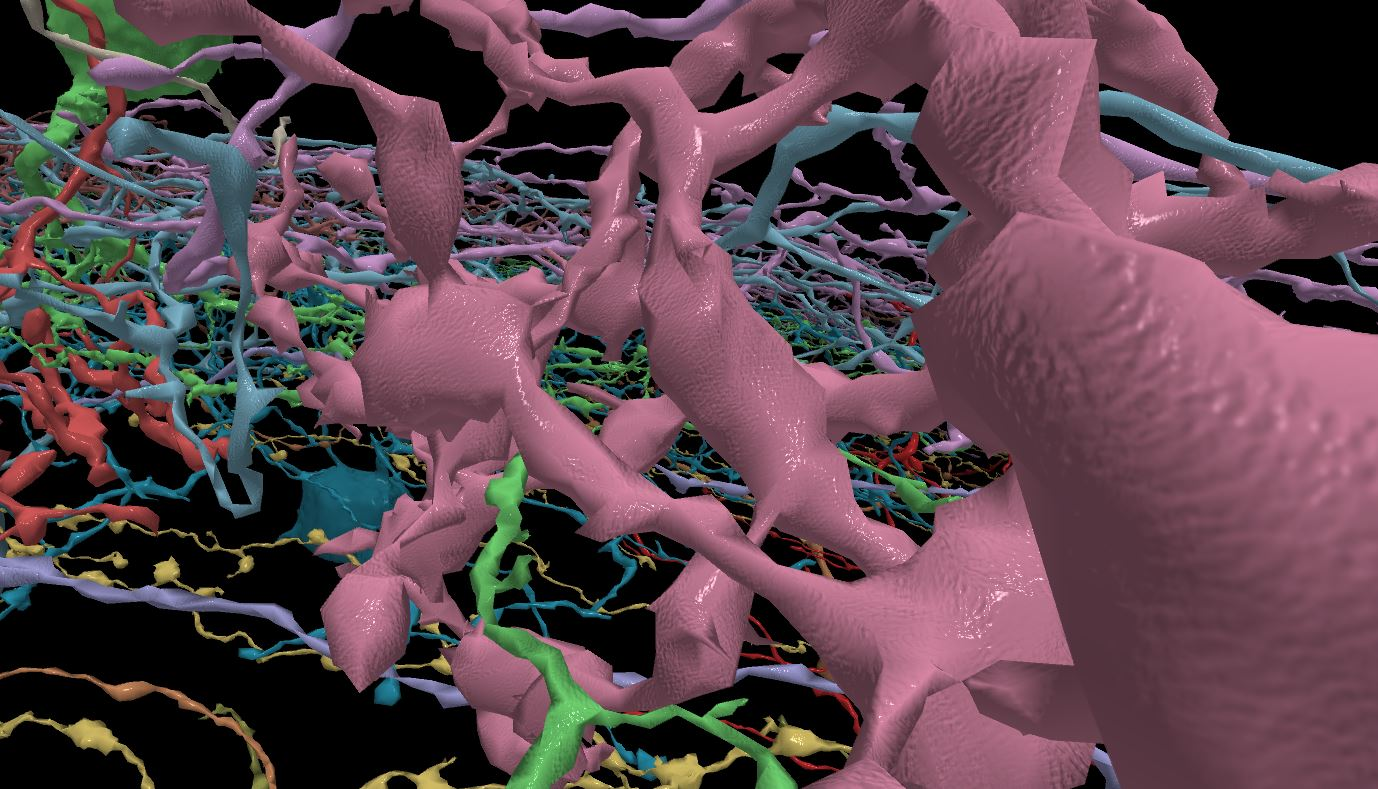
\includegraphics[width=1.0\linewidth]{gen.png}
\end{center}
   \caption{Rendering neuron connection with mesh. The colors for each neuron in the mesh vertices has been encoded.A technique called tri-planar texture mapping has been used to add a normal map without using UV coordinates, giving the models a shiny/bumpy look up close.}
\label{fig:long}
\label{fig:onecol}
\end{figure}

This project[x] has reported a novel approach to trace neuronal circuits in brain. It is a interdisciplinary research which provides a solution for connectomics researchers with virtual reality technology. The main goal of this project is to improve the quality and speed of neuron tracing, This is achieved with different innovative rendering, interaction, and navigation methods provided by the author. There are some similar projects like The Virtual Finger in Vaa3D and NeuroLucida 360. These methods provides semi-automatic extraction approaches which improves the speed at which neuron morphology can be traced.But they are viewpoint and visibility dependent. Which means that they can be very slow when the data size increases. Also, Jeong et al. combine segmentation and stitching analysis with an out-of-core GPU volume renderer for large datasets.
\subsection{Rendering}
Difficulties in rendering neuron with HMDs are found in state-of-art methods.It presents a significant challenge to avoid motion sickness with both high-resolution and frame-rate requirements. Low frame rates and pauses during computation are not as tolerable as the case in traditional desktop visualization. With HMDs, we have a limited time to render each frame, which is only about 11ms. Compared to our VRAM of current GPUs(4-24GB) and RAM(64-128GB) space in our computers, the neuron datasets can be very large, range from hundreds of gigabytes to terabytes. Thus, we need to work with data stream. It is reported in this project that only 2ms is budgeted for data streaming on the render thread, which is very short. Moreover,it is common to step inside the dataset. When walking through the 
volume, it is observed that the scene begin to vibrate, this should be eliminated for a better experience.After that, We need to correctly composite the geometry, wands, and tracings when using volume rendering technique. At the same time, Depth perception can be challenging in volume rendering, when we just use gradient shading. Thus, it might hard to determine the exact position of the wands in this case. When enhance the depth perception using isosurface rendering mode, if the data is noisy, the result is not ideal.

The author of this paper has presented novel approaches to solve the problems above. To avoid motion sickness they take cues from VR game development. They have designed a streamlining rendering pipeline, in which they submit draw calls approximately equal to 2ms before VSync. At the same time, the asynchronous volume data will be uploaded based upon the user’s focus region instead of the whole scene. It is a strictly budgeting work which improves the rendering performance significantly. To deal with huge amount of data with a limited rendering time, they provided a data streaming solution. At the same time, they use a two-level caching system in it: the first level loads and caches pages from disk into RAM, and the second level takes these pages and uploads them to the GPU. A faster data loading process can be achieved by reducing disk access frequency and latency to display pages with the caching system above. On an other hand, they presents a scheme to restrict the visible popping of pages. That is, they load a box slightly larger than the focus region and prioritize pages closer to the user’s view. This scheme of limiting the enqueueing rate has been found simpler than updating priorities for already scheduled pages. To avoid vibrate effect when wandering across the datasets, they begin sampling at the sample point nearest to the clipping plane. To do composition correctly, In the raymarching step, they use the depth buffer produced by rendering the opaque geometry to terminate rays early. Moreover, Shadows or global illumination which are advanced rendering techniques that can improve the perception of depth. But those techniques are computational expensive, and hard to apply in a VR setting if we want to maintain a sufficient frame rate for VR. The author of this paper does not use those techniques due to their significant frame-rate or memory cost. Instead, they added the ability to switch to an implicit isosurface mode, with Phong shading and ambient occlusion. To deal with noisy data in the implicit isosurface mode, they de-noise the data first. More precisely, they filter out objects less than 11 voxels in size before uploading the page to the GPU by finding small connected components.

\begin{figure}[h]
\begin{center}
%\fbox{\rule{0pt}{2in} \rule{0.9\linewidth}{0pt}}
   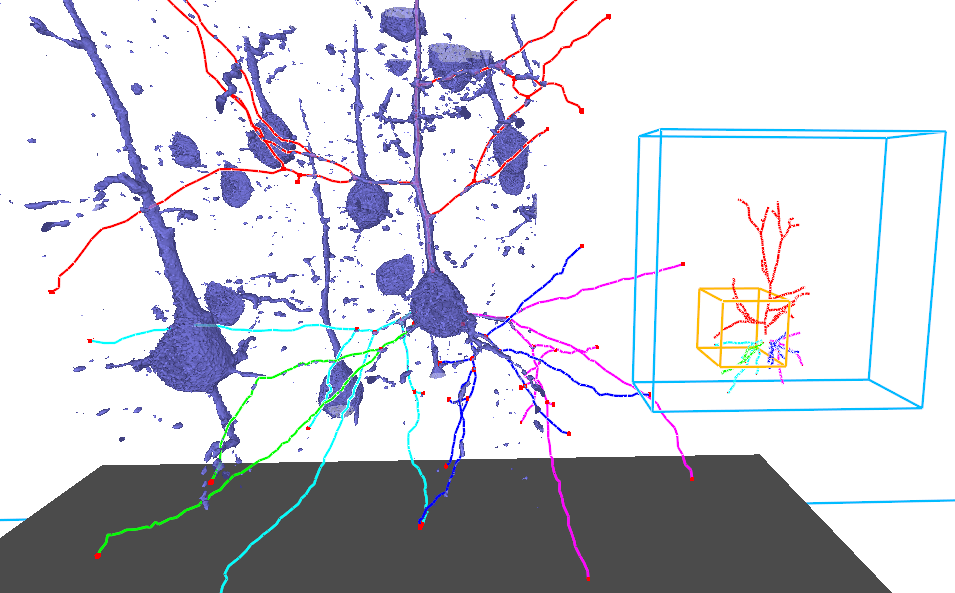
\includegraphics[width=1.0\linewidth]{neuron-render.png}
\end{center}
   \caption{A screenshot of the system, using the isosurface rendering mode. With the help of minimap (right), Users can orient themselves in the dataset. It shows the world extent in blue, the current
focus region in orange, and the previously traced neuronal structures.}
\label{fig:long}
\label{fig:onecol}
\end{figure}

\subsection{Interaction}
Tracing and navigation are key tasks when reconstructing neurons. Difficulties can be found in state-of-art methods to achieve this. There is a problem when designing the interaction model: what to use and how to use interaction tools. If we have designed something that hard to navigate through the dataset, it will be less powerful when used by experts from the field of neuron research. Besides, We have to make sure that the correctness of tracing the branches of a neuron can easily be achieved. That means, the tracing of branches must be easy to do. Additionally, It is always a good idea to give feedback to the user during the interaction in a system.Thus, we have to call attention to the user when they are trying to select something.

\begin{figure}[h]
\begin{center}
%\fbox{\rule{0pt}{2in} \rule{0.9\linewidth}{0pt}}
   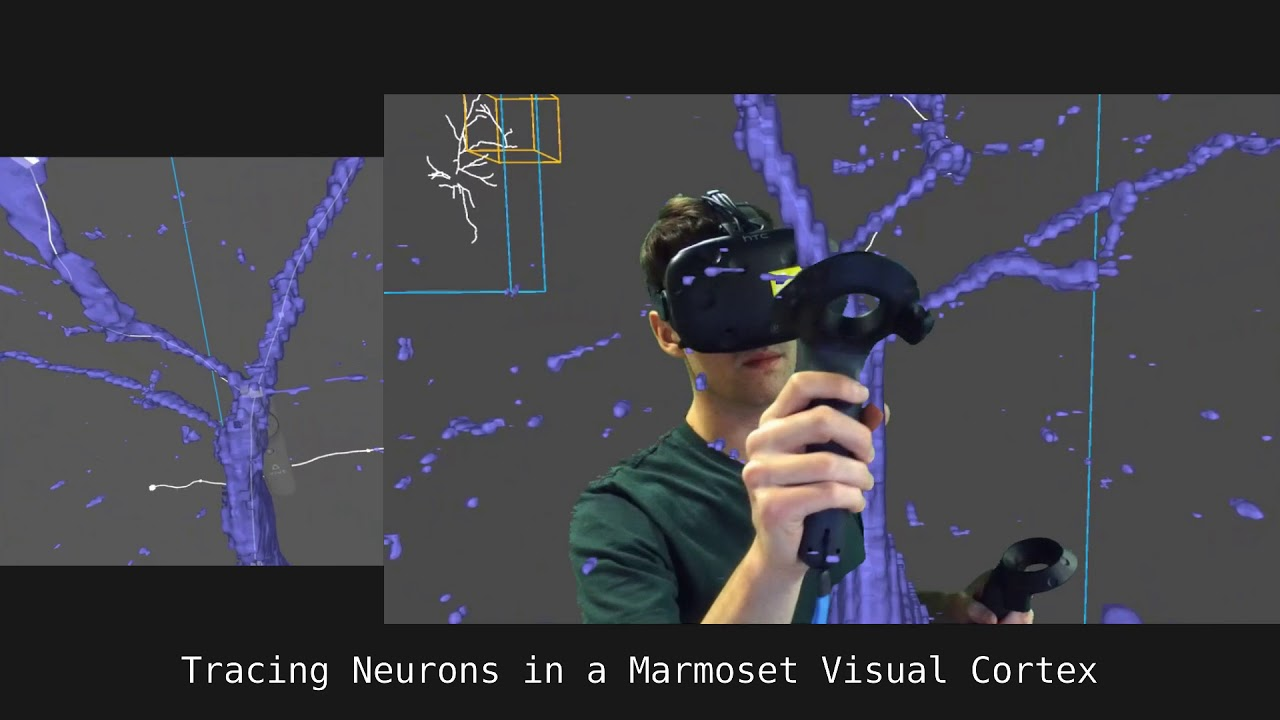
\includegraphics[width=1.0\linewidth]{neurou-tracing.png}
\end{center}
   \caption{Navigating through large-scale dataset using VR controller: navigation wand. That handheld controller also enables us throwing, steering and aiming in VR scene.}
\label{fig:long}
\label{fig:onecol}
\end{figure}

\begin{figure}[h]
\begin{center}
%\fbox{\rule{0pt}{2in} \rule{0.9\linewidth}{0pt}}
   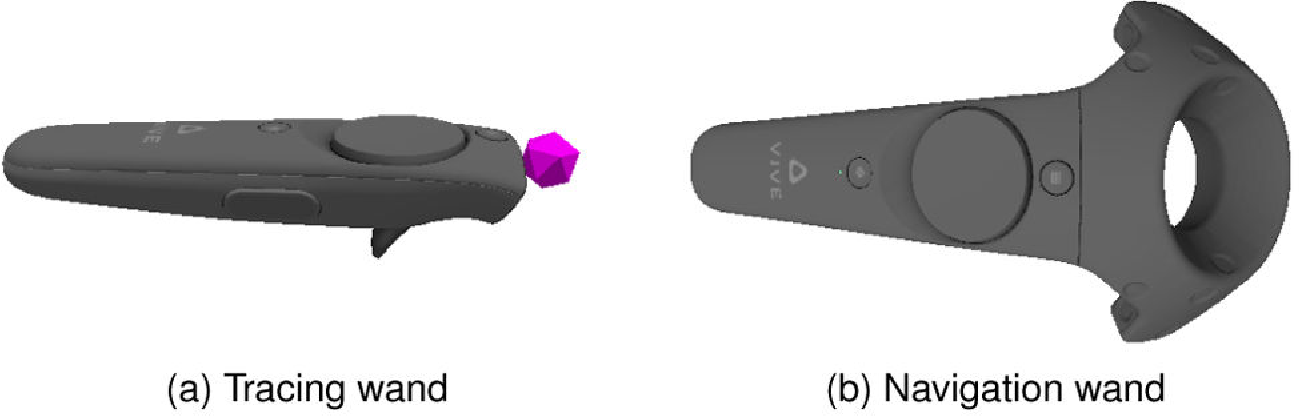
\includegraphics[width=1.0\linewidth]{wands.png}
\end{center}
   \caption{The button sticking out underneath (a) is
the trigger, and the large circular button is the trackpad. The icosphere
brush in (a) is colored to match the selected line color.}
\label{fig:long}
\label{fig:onecol}
\end{figure}

In this project, they use the wand model with two wands: One is used for tracing and the other for navigation. The actions are initiated by holding the trigger button on the corresponding wand to avoid spurious triggering. The navigation wand is rendered to match the wand’s physical model to avoid motion sickness. The user then holds the trigger she or she follows the neuron through the data, drawing a line from the brush. Releasing the trigger ends the line and creates the termination point. The user is then free to continue the line from the termination point, or trace branches as needed. This is the key interaction process designed in that paper. It makes users easier to navigate large dataset, which motivates users to work in a immersive way and have a better understanding of it at the same time. The creation of a branch in their system is easy, by letting users to select different drawing methods instead of just one. The user can start a new line along the current tracing and follow the neuron branch out, or start a new line on the neuron branch and reconnect to the parent tree. To call attention to the reconnection, they highlight the selected node and send a small vibrationto the wand to give a “click” feeling of selecting it. Also, they display a small cube to indicate where the branching point will be placed. The visual and physical feedback provides a clear signal to the user that the desired operation has been done. By importing those feedback methods, the interaction between the user and the system is enhanced.
\section{Molecular Visualization}
\subsection{Overview}
Molecular visualization in virtual reality can be useful for visualizing and analyzing molecular structures and three-dimensional (3D) microscopy by providing intuitive perception of complex structures. Virtual reality (VR) offers immersive display with a wide field of view and head tracking for better perception of molecular architectures and uses 6-degree-of-freedom hand controllers for simple manipulation of 3D data. Which helps scientists to gain a better understanding of their data. The increase in the knowledge of macromolecular structures lets scientists to understand the real world better. Software packages for this purpose can easily be found. Such as VMD,a well-known molecular visualization program for displaying, animating and analyzing large biomolecular systems using 3D graphics and built-in scripting. PyMOL, a Python-enhanced molecular graphics tool that normally runs on desktop machines. But most of them only work on a desktop PC. Nowadays consumer VR headsets are affordable to researchers and educators. Thus, pushing the scientific visualization applications to virtual reality environment has becomes a research topic. However, due to the need for low-latency, high-frame-rate rendering, it is challengeable to be realized in HMDs without so-called simulator sickness. At the same time, new interaction problems should also be solved.

\begin{figure}[h]
\begin{center}
%\fbox{\rule{0pt}{2in} \rule{0.9\linewidth}{0pt}}
   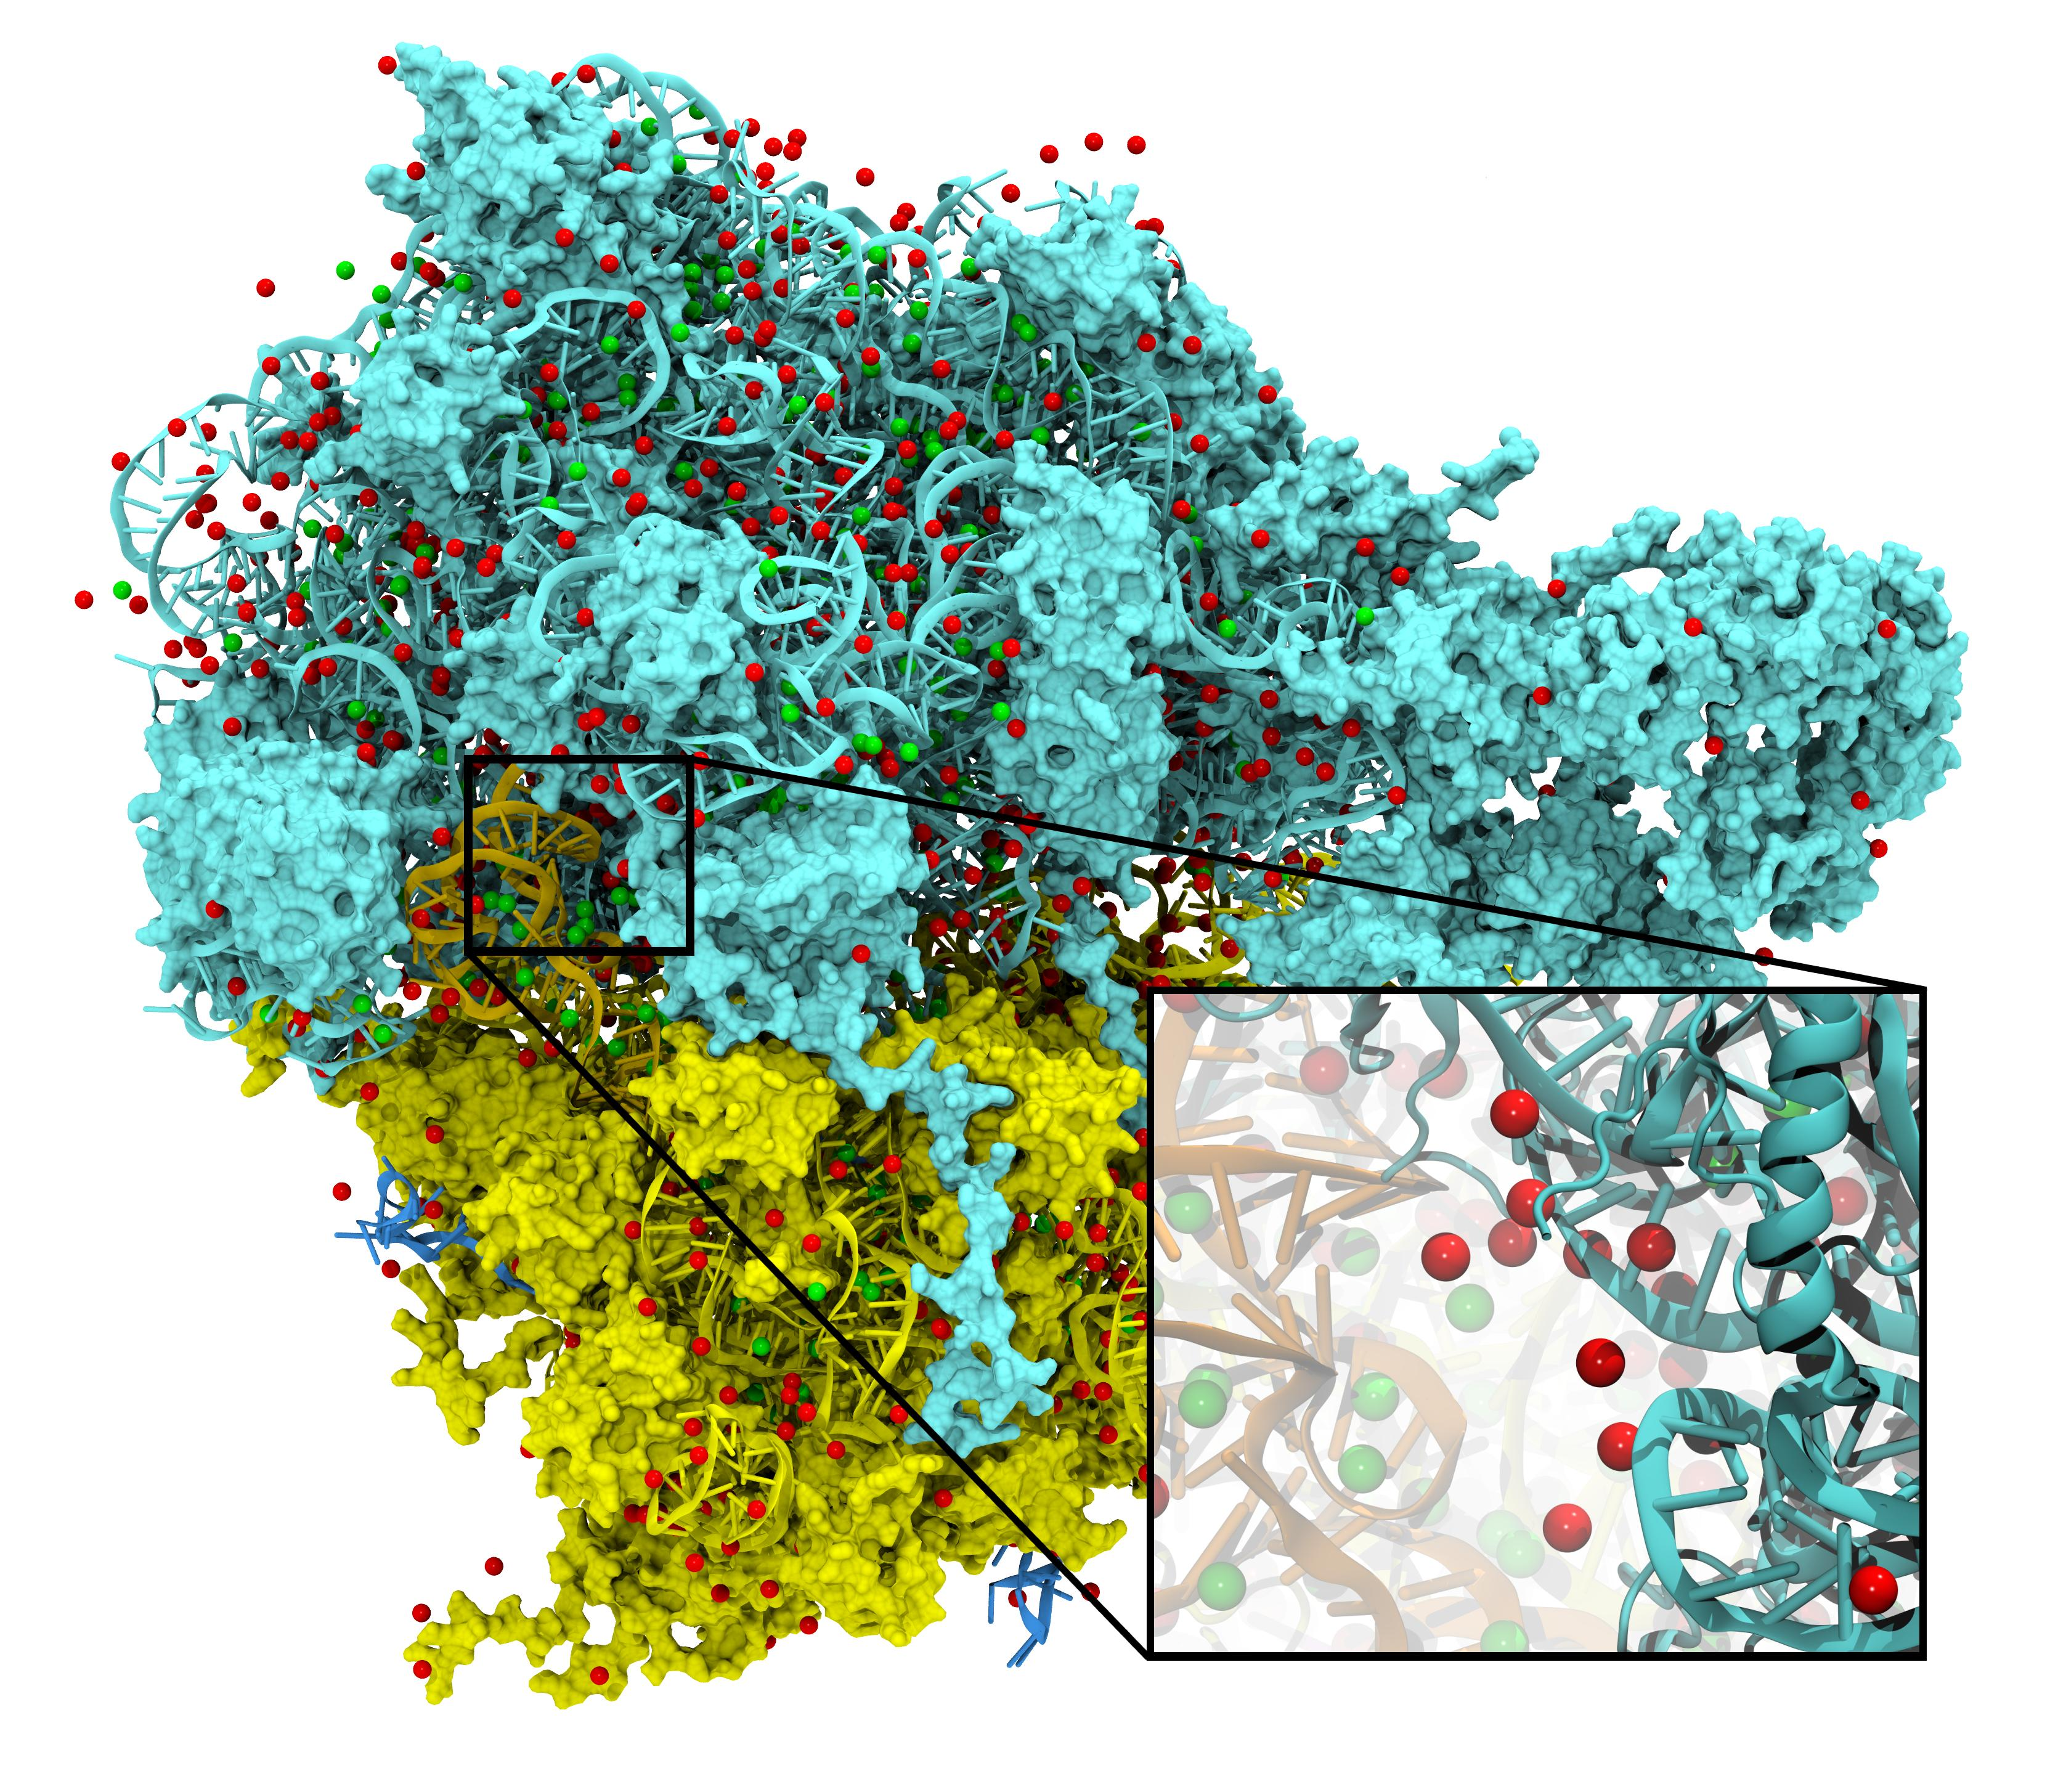
\includegraphics[width=1.0\linewidth]{complex-structure.jpg}
\end{center}
   \caption{The visualization of large bacterial ribosome structure.}
\label{fig:long}
\label{fig:onecol}
\end{figure}

In this project[x], researchers provides a novel solution for molecular visualization with head mounted displays(HMDs). Which achieves the performance levels required for comfortable use of HMDs while dealing with large-scale datasets and network latencies when viewing with the help of a remote server. Similar projects can also be found. But this project combines immersive visualization techniques with high quality progressive RT( implements advanced techniques such as ambient occlusion lighting, depth of field focal blur )and supports remote rendering scenarios while achieving frame rates suitable for use in virtual environments. 

\subsection{Remote Visualization and The System Design}

Difficulties can be found in state-of-art immersive molecular visualization solutions in the rendering process. The data size and computing requirements for effective visualization will increase all the time because of the continue growing size and timescale obtained by experimental imaging. Regular transfer of such large amounts of data is impractical. Thus, we have to deal with large-scale datasets. When using remote visualization to eliminate the need for large file transfers, there will be a new problem: round-trip network latencies. Which would cause simulator sickness when using HMDs. Moreover, when using data streaming technique, best H.264 video encoding parameters should be found. Besides, the architecture of the system should be carefully designed.

To overcomes network latencies, they present a novel two-phase rendering approach works with the combination of omnidirectional stereoscopic progressive ray tracing and high performance rasterization. They implemented that based on VMD. The system provides high-fidelity rendering previously inaccessible within immersive visualization systems. Hardware-accelerated video encoding has profoundly increased frame rates and image resolution for remote visualization. They find that the best frame rate is achieved using a single 8-GPU VCA nod.System for remotely-rendered immersive molecular visualization with HMDs designed to be a collection of components and data flow. Their system uses multithreading to maintain asynchronous execution of progressive RT and HMD display updates, with the HMD view update loop and user input handling residing in the main VMD thread.

\subsection{Rendering and Displaying Techniques}

During the rendering process, advanced rendering techniques(such as shadows, ambient occlusion lighting,depth-of-field, and high quality transparency) should also be implemented to facilitate the study of large biomolecular complexes. Speckle noise can be found in many AO lighting approximations. Uncorrelated AO sampling produces high quality converged images, but creates strong pixelated speckle noise until the image approaches convergence with a large number of accumulated samples.Again, problems has been found when accelerating with multiple GPUs. Parallel efficiency is limited by uneven work distribution in different regions of the rendered scene. During the process of omnistereo and panoramic ray tracing of biomolecular scenes, the standard planar formulations should be reimplemented with radial or spherical formulations. Including depth-of-field focal blur, fog and depth cueing, as well as view frustum clipping. In the rendered scene, The crowded molecular environment can be a dark place due to heavy shadowing with both AO and direct lighting. Which should also be fixed. When viewing with DK2 and similar HMDs, the singlet ocular lenses produce strong pincushion geometric distortion. Thus, distortion correction software should be implemented. Additionally, The 75 Hz display refresh rate of the DK2 should be achieved to provide a smoothest immersive visualization experience.

\begin{figure}[h]
\begin{center}
%\fbox{\rule{0pt}{2in} \rule{0.9\linewidth}{0pt}}
   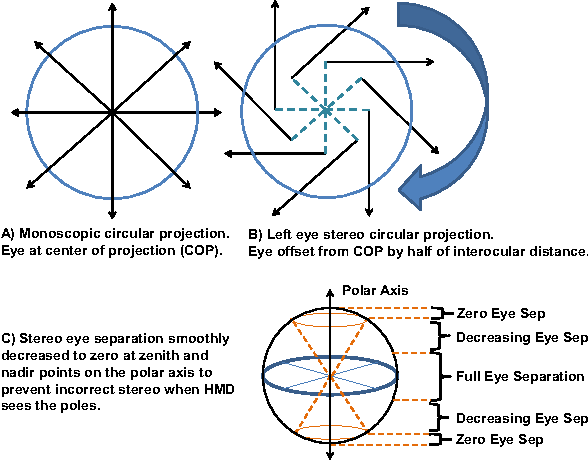
\includegraphics[width=1.0\linewidth]{projection-approach.png}
\end{center}
   \caption{The omnidirectional stereoscopic projection approach.}
\label{fig:long}
\label{fig:onecol}
\end{figure}

To accelerate the rendering process with advanced technique such as ambient occlusion lighting, fog and depth cueing, and depth of field focal blur, they have introduced a new ray tracing algorithm used to optimize interactivity and quality. And a projection approach that supports widely used spherical and cubic texture mapping operations in commodity graphics hardware. They also design and implementation a high performance progressive RT engine based on data-parallel CUDA. Direct lighting often act to obscure features of molecular structure without careful light placement while computationally inexpensive. To support advanced lighting effect for a better experience of users, they improved their progressive ray tracing algorithm. As a result, the rendering engine produces high quality images. Their RT algorithm has been accelerated using techniques like CUDA, OpenCL, ISPC, and IVL, with the help of highly parallel SIMD-oriented hardware architectures. To support video streaming, they extends the TachyonLOptiX GPU-accelerated RT engine to combine video streaming technique. To get a higher performance, they update the displayed image by launching and accumulating one ormultiple images, so-called “subframes”, in each iteration. A progressive RT engine customized for immersive molecular visualization has been implemented to employ the newly designed RT. To deal with speckle noise mentioned above, they use a single random number stream to drive AO sampling for all pixelsin the same subframe. In this way, all pixels take AO lighting samples in the same direction, thereby eliminating speckle noise. The flutter effect has been eliminated. For they use a moving average to track its update rate and dynamically adjust the number of samples computed by successive subframes with the goal of maintaining a target update rate. Once the number of subframe samples has been determined, the progressive RT engine chooses a sample allocation strategy that favors image-space refinement. They found that tens of GPUs can be effectively utilized for interactive progressive rendering of complex scenes. To deal with the darkness problem, they added a point light “headlight” at the center of projection to prevent excessive darkening when viewing interiors of fully-enclosed organelles. But it produces “flat” looking shading since it is very close to the camera position. For this, they modified the AO shadow test algorithm to ignore shadows from occluding geometry beyond a maximum radius from the hit point. Thus, AO lighting can be effectively used. When displaying, their RT engine can produce a variety of omni-stereo projections including latitude-longitude,cube map and dome-master. They also developed HMD display and distortion correction software optimized both for the stock DK2 HMD and for DK2 HMDs with enhanced ocular optics. Pincushion distortion mentioned above can be neutralized by applying the inverse barrel distortion prior to display. To increase the update rate during the displaying process, they use a variety of techniques to implement an HMD display loop. After that, HMD update rates can exceed 100 Hz (10 ms redraw interval) on commodity PC hardware. Where the RT engine and HMD display update loops run asynchronously in independent threads. To prevent the HMD display update loop from monopolizing the host CPUs, the display GPU, and the host PCIe bus, they make the update loop blocks on a final OpenGL buffer swap. When achieving higher performance using a host machine with slower CPUs, they developed a routine to eliminate redundancy during the upload of OpenGL textures. The worst case HMD update interval has been reduced in this way.

\subsection{Interaction}
Uncomfortable stereoscopic views can be caused when structures are too close to the camera. Which makes navigation difficult. Rendering options should be displayed in the scene to enhance the interaction process.

To solve the navigation problem above, an optional clipping sphere feature was added to their RT engine. Objects inside the sphere (near the viewer’s eyes) are smoothly faded toward complete transparency and are ultimately clipped out entirely. To prevent clipped geometry from casting shadows, the clipping sphere also affects secondary rays. They provide the user with graphical information in the form of heads-up display(HUD) and have drawn special avatar geometry that represents the user’s wand.
{\small
\bibliographystyle{unsrt}
\bibliography{reviewbib}
}

\end{document}
